\documentclass[11 pt]{article}

\usepackage{amsmath}
\usepackage{fancyhdr}
\usepackage[left=2cm,right=2cm,top=2cm,bottom=2cm]{geometry}
\usepackage{graphicx}
\usepackage[hidelinks]{hyperref}


\pagestyle{fancy}
\fancyhf{}
\lhead{Fundamentals of Simulation Methods}
\chead{Exercise 03}
\rhead{V. Mader}
\setlength{\headheight}{15pt}


\begin{document}

    \section{Order of ODE integration scheme}
    ...

    \section{Integration of a stiff equation}
    Consider a radiatively cooling ionized plasma of hydrogen gas. \\
    The temperature evolution is governed by
    \begin{equation}
        \frac{dT}{dt}=-\frac{2}{3k_B}n_H\Lambda(T)    
    \end{equation}
    where $\Lambda(T)$ describes the cooling rate as a function of 
    temperature, which is approximated by 
    \begin{equation}
        \Lambda(T)=
        \begin{cases}
            \Lambda_0(\frac{T}{T_0})^\alpha\textnormal{ for }T\leq T_0 \\
            \Lambda_0(\frac{T}{T_0})^\beta\textnormal{ for }T>T_0
        \end{cases}
    \end{equation}
    \paragraph{Determine the temperature evolution $T(t)$ by integrating 
    the differential equation with a second-order Runge-Kutta 
    predictor-corrector scheme and a fixed timestep, until the 
    temperature has dropped below $6000$ K. Use a timestep size of 
    $\Delta t=10^{10}$ s. Make a plot of the time evolution of the temperature,
    with a logarithmic scale for temperature and a linear scale for time.} \ \\
        \begin{figure}[h!]
            \centering
            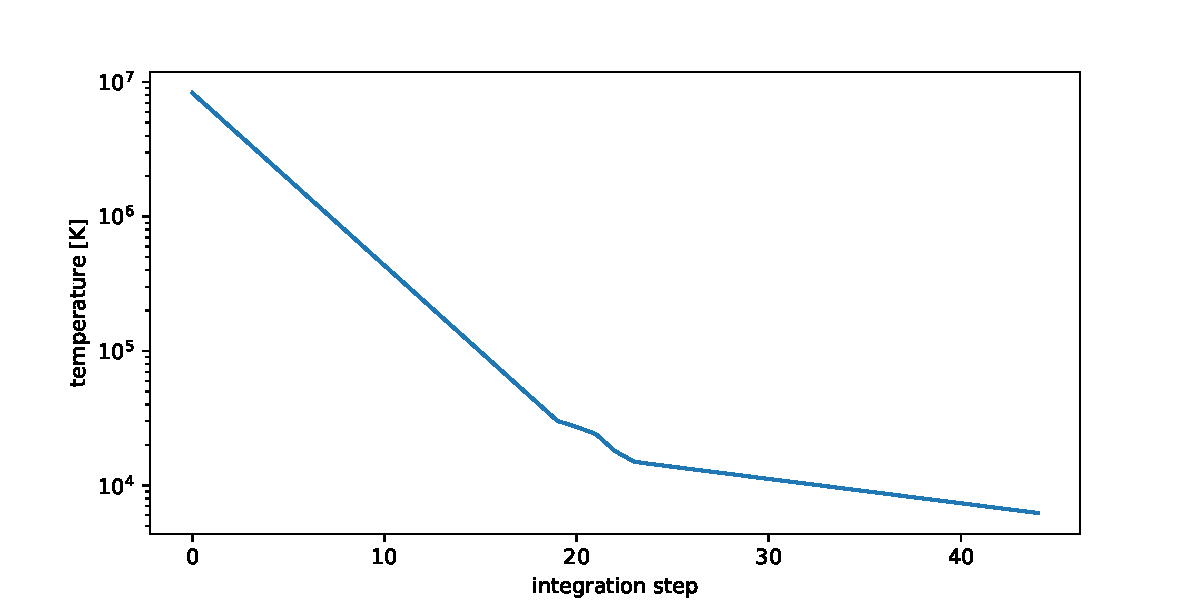
\includegraphics[width=0.8\linewidth]{temperatures.pdf}
        \end{figure}

    \paragraph{How many steps do you roughly need to reach the final 
    temperature?} \ \\ 
    \\
        I am not quite sure what is meant with "final temperature",
        since the temperature continues to drop even after $T$ 
        crosses $T_0$. The slope becomes much less steep though, so 
        one might say that the "final temperature is reached"
        at this point.

    \newpage\noindent
    % \paragraph{Now implement the second-order integration from a) with an 
    % adaptive step size control, based on estimating the local truncation 
    % error by carrying out two half-steps for every step. Use a local error
    % limit $\Delta T_\textnormal{err}^\textnormal{max}=50$ K for every step.
    % Overplot your result for the temperature evolution, on the plot for a),
    % using symbols or a different color. How many steps do you now need?
    % Confirm that your scheme is robust to large changes of the timestep-size 
    % given as input for the first step.} \ \\
    % ...

    \section{Double pendulum}
        \noindent Lagrangian:
        \begin{align}
            L=
            &\frac{m_1}{2}(l_1\dot{\Phi}_1)^2+
            \frac{m_2}{2}\bigg[
                (l_1\dot{\Phi}_1)^2+
                (l_2\dot{\Phi}_2)^2+
                2l_1l_2\dot{\Phi}_1\dot{\Phi}_2\cos(\Phi_1-\Phi_2) \\
            &-m_1gl_1(1-\cos{\Phi_1})-m_2g[l_1(1-\cos{\Phi_1})+l_2(1-\cos{\Phi_2})]
            \bigg]
        \end{align}
        For later, we define $M=m_1+m_2$ and $\Delta\Phi=\Phi_1-\Phi_2$.

        \paragraph{a) Derive the Lagrangian equations of motion} \ \\
        \\
        We set 
        \begin{align}
            q_1
            &=\frac{\partial L}{\partial\dot\Phi_1}
            =m_1l_1^2\dot\Phi_1+m_2l_1^2\dot\Phi_1
            +m_2l_1l_2\dot\Phi_2\cos(\Phi_1-\Phi_2) 
            \label{eq:bla} \\
            % \Rightarrow \dot\Phi_1
            % &=\frac{q_1-2l_1l_2\dot\Phi_2\cos(\Phi_1-\Phi_2)}{(m_1+m_2)l_1}
            \\ q_2
            &=\frac{\partial L}{\partial\dot\Phi_2}
            =m_2l_2^2\dot\Phi_2
              +m_2l_1l_2\dot\Phi_1\cos(\Phi_1-\Phi_2) 
            \label{eq:blu} \\
            % \Rightarrow \dot\Phi_2
            % &=\frac{q_2-2l_1l_2\dot\Phi_1\cos(\Phi_1-\Phi_2)}{m_2l_1}
        \end{align}
        For $\Phi=\Phi_1$:
        \begin{align}
            0
            &=\frac{d}{dt}\frac{\partial L}{\partial\dot\Phi_1}
            -\frac{\partial L}{\partial\Phi_1} \\
            &=\frac{dq_1}{dt}+\bigg(
                m_1gl_1\sin{\Phi_1}+m_2gl_1\sin{\Phi_1}
            \bigg) \\
            \Rightarrow\frac{dq_1}{dt}&=-(m_1+m_2)gl_1\sin\Phi_1
            % -m_1gl_1\sin{\Phi_1}-m_2gl_1\sin{\Phi_1}
        \end{align}
        For $\Phi=\Phi_2$:
        \begin{align}
            0
            &=\frac{d}{dt}\frac{\partial L}{\partial\dot\Phi_2}
            -\frac{\partial L}{\partial\Phi_2} \\
            &=\frac{dq_2}{dt}+\bigg(
                m_2gl_2\sin{\Phi_2}
            \bigg) \\
            \Rightarrow\frac{dq_2}{dt}&=-m_2gl_2\sin{\Phi_2}
        \end{align}

        \paragraph{Cast the system of equations into 1st-order form
            $\frac{d}{dt}\vec y=\vec f(\vec y)$
        } \ \\
        \\
        We set
        \begin{equation}
            \vec y=(\Phi_1,\Phi_2,q_1,q_2)^T
        \end{equation}
        % \begin{equation}
        %     \vec f(\vec y)=\frac{d}{dt}\vec y
        % \end{equation}
        % We can rearrange \autoref{eq:blu} to get $\dot\Phi_2$ and then plug it 
        % into \autoref{eq:bla}. Then we can again rearrange so that we get 
        % $\dot\Phi_1$, which will be used to define $f_1$. $f_2$ can then 
        From \autoref{eq:bla} and \autoref{eq:blu} we get
        \begin{align}
            \Rightarrow\dot\Phi_1
            &=\frac{q_1-m_2l_1l_2\dot\Phi_2\cos(\Delta\Phi)}{Ml_1^2} \\
            \Rightarrow\dot\Phi_2
            &=\frac{q_2}{m_2l_2^2}-\frac{l_1}{l_2}\dot\Phi_1\cos(\Delta\Phi)
        \end{align}
        Now we know everything we need to define $f$:
        \begin{align}
            f_1&=\dot\Phi_1=
            \frac{q_1-m_2l_1l_2\dot\Phi_2\cos(\Delta\Phi)}{Ml_1^2} \\
            f_2&=\dot\Phi_2=
            \frac{q_2}{m_2l_2^2}-\frac{l_1}{l_2}\dot\Phi_1\cos(\Delta\Phi) \\
            f_3&=\dot{q}_1=-m_1gl_1\sin{\Phi_1}-m_2gl_1\sin{\Phi_1} \\
            f_4&=\dot{q}_2=-m_2gl_2\sin{\Phi_2} \\
        \end{align} 

        \paragraph{Write a computer program that integrates the system with 
        a second order predictor-corrector Runge-Kutta scheme.} \ \\
        \\
        Plotting the energy leads to the following graph:
        \begin{figure}[h!]
            \centering
            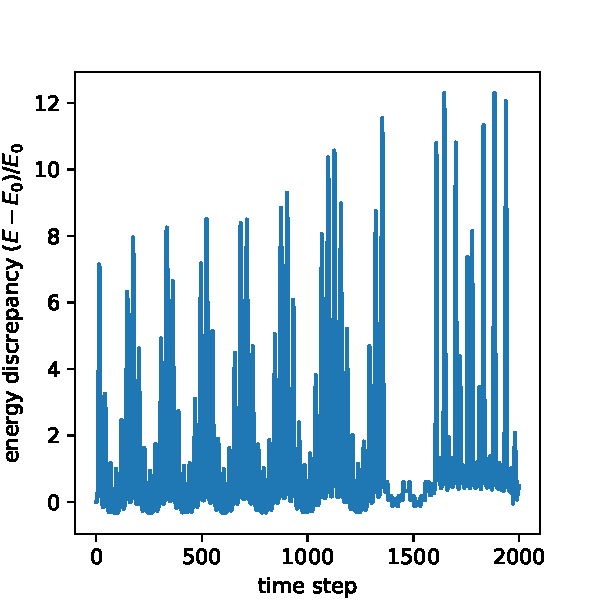
\includegraphics[width=.5\textwidth]{./energies_rk23.pdf}
        \end{figure} \ \\
        As can be seen clearly, the energy is not conserved. I am not 
        sure whether this is expected or whether I made an error 
        while rearranging the equations. There also is a periodic 
        structure in the energy deviation.

        \newpage\noindent
        \paragraph{Produce a second version of your code using a fourth-order
        Runge-Kutta algorithm.} \ \\  
        \begin{figure}[h!]
            \centering
            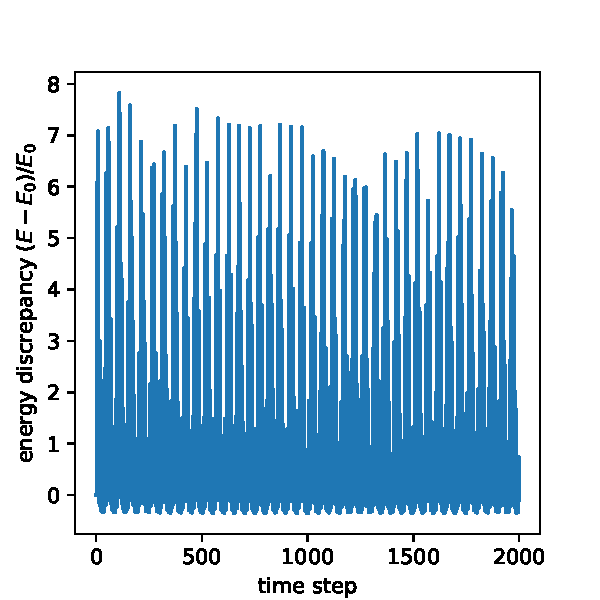
\includegraphics[width=.5\textwidth]{./energies_rk45.pdf}
        \end{figure} \ \\ 
        Once again, the energy is not conserved, but this time the 
        deviation from $E_0$ is smaller.


\end{document}
